\chapter{Architecture}

\begin{figure}[!h]
\begin{center}
  \fbox{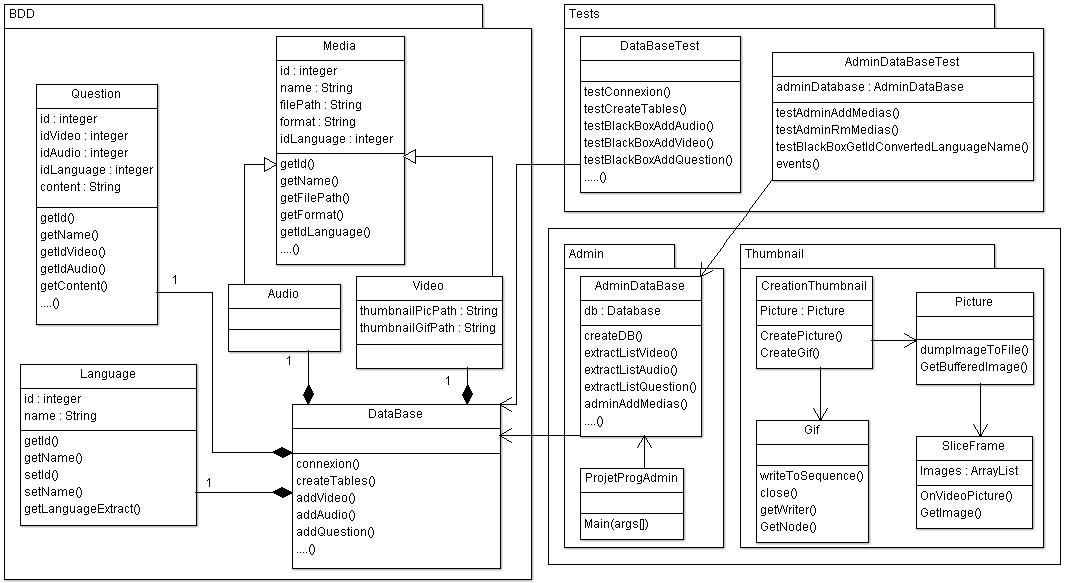
\includegraphics[width=25cm,angle=90]{./architecture/UML-MA.png}}
  \caption{UML - Architecture du modèle et de l'administration ainsi que des test}
  \label{archi} 
\end{center}
\end{figure}

\begin{figure}[!h]
\begin{center}
  \fbox{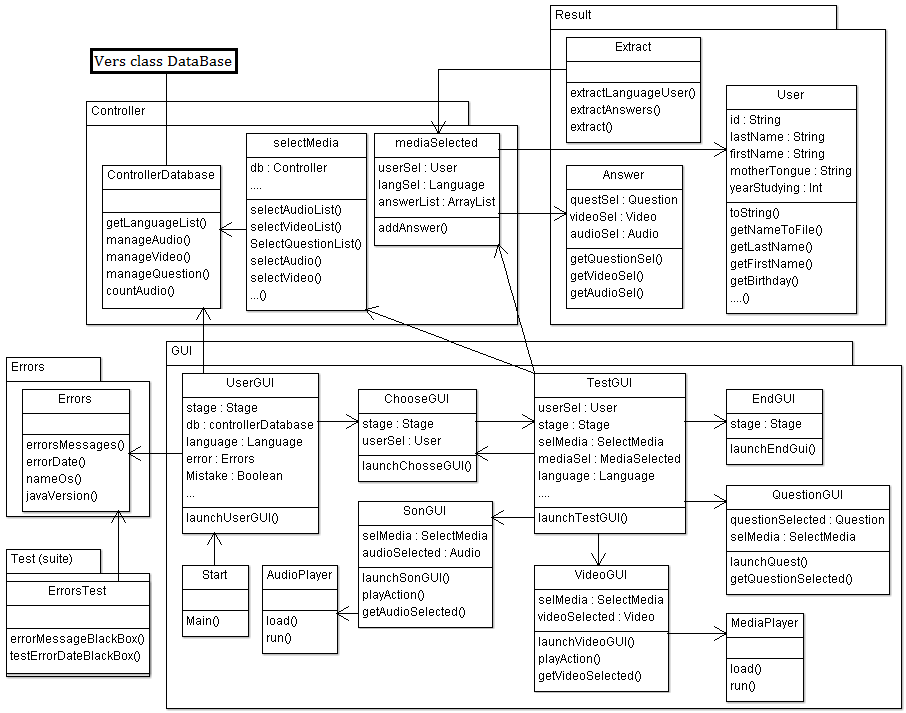
\includegraphics[width=22cm,angle=90]{./architecture/UML-VCU.png}}
  \caption{UML - Architecture du controlleur, de la vue et du résultat ainsi que des errors}
  \label{archi} 
\end{center}
\end{figure}

L'architecture \textbf{M}odele-\textbf{V}ue-\textbf{C}ontroleur (\textbf{MVC}) permettant "la séparation des éléments principaux d'un système d'intéraction d'une couche présentation" \footnote{Citation du cours magistral de PdP de M.Narbel} nous semblait le pattern le mieux adapté au développement de notre application basée sur les liens base de données/interface graphique. 

De plus, grâce à ce \textit{design pattern}, nous avons pu répartir les rôles de chacun afin de produire un travail efficace.

\section{Application principale}

Notre architecture est structurée en plusieurs packages. Ils ont été créés pcompartimenter notre architecture en fonction des besoins renseignés précédemment. Chaque package regroupe un certain nombre de classes, chacune possédant une fonction bien précise.

Dans cette section, nous allons décrire le besoin que nous avons voulu satisfaire avec chaque package et le rôle de chacune de leurs classes. Pour suivre la logique MVC, nous allons structurer la description selon ce même pattern.


\subsection{BDD}

Ce package concerne tout ce qui se rapproche de la base de données. Ainsi, il possède tous les types d'objet que nous allons insérer et sélectionner :
\begin{itemize}
 \item \textit{Media} :
 \begin{itemize}
  \item \textit{Video}
  \item \textit{Audio}
 \end{itemize}
 \item \textit{Language}
 \item \textit{Question}
\end{itemize}
Ces types d'objet intéragissent avec la base de données via la classe \textit{Database}.


\subsubsection{Classe DataBase}

Cette classe contient toutes les intéractions entre les objets et la base de données (on notera BDD dès à présent). Elle permet de :

\begin{itemize}
 \item se connecter à la BDD (créer et initialiser la BDD le cas échéant)
 \item remplir la BDD
 \item rechercher dans la BDD
 \item supprimer des éléments dans la BDD
 \item consulter la BDD
\end{itemize}

Cette centralisation permet d'optimiser l'accès à la BDD, faciliter la gestion de conflits et gérer les échanges de médias tout au long de l'application.

\subsubsection{Classes Media, Audio et Video}

Ces trois classes sont unies : les classes \textit{Audio} et \textit{Video} héritent de la classe abstraite \textit{Media}. Cette dernière regroupe les méthodes communes aux classes héritées. Ce pattern nous est utile vu qu'il nous permet de fusionner un code redondant. Ces classes Audio et Video créent des objets par rapport aux champs de la base de données. Ce choix nous permet d'éviter de nombreuses connexions inutiles avec la BDD, coûteuses en temps.

\subsubsection{Classe Question, Language}

Ces classes créent des objets correspondants à une question et à une langue issues de la base de données.
Les objets \textit{Question} ne sont utiles qu'à l'administrateur puisque le sujet n'a besoin que du contenu.
Les objets \textit{Language} nous permettent de sélectionner audios, vidéos et questions soumis aux sujets.

\subsection{Controller}\label{archi_controller}

Dans une architecture MVC, le controller sert de lien entre la partie modèle et la partie vue. Il va chercher les différents objets du modèle utiles à la vue et modifie, si besoin, les objets que la vue a manipulé.

\subsubsection{ControllerDatabase}

Cette classe fait le lien entre le modèle et la vue, c'est elle qui récupère les méthodes du modèle pour les utiliser dans la vue, et inversement. Ces méthodes n'affectent pas directement la vue, car elles sont utilisées par les deux autres classes du package pour générer des objets de média voulus.
Cette classe est importante vu qu'elle est le lien vers la classe \textit{Database}. A chaque fois qu'un objet souhaite accéder aux données, cette classe est là pour "abstraire" la classe Database. En effet, le sujet ne manipule pas directement celle-ci. Ce choix offre une sécurité supplémentaire sur la classe la plus importante de notre projet.

\subsubsection{SelectMedia}

Cette classe sélectionne, de manière aléatoire, les questions, les vidéos et les audios auxquels le sujet sera soumis lors du test.

\subsubsection{MediaSelected}

Cette classe permet de récupérer les différentes informations nécessaires à l'exportation, via le package \textit{Result} (voir \ref{Archi_Results}). Ces informations sont multiples : les divers renseignements que l'utilisateur a entré, la langue du test, les questions soumises lors de celui-ci ainsi que les medias sélectionnés par l'utilisateur.


\subsection{GUI}\label{modele}

Dans une architecture MVC, ce package correspond au terme "vue". Il regroupe toutes les configurations et les fonctionnalités de l'interface graphique.

\subsubsection{Classe Start}

C'est à partir de cette classe que l'application se lance.
Cette classe permet de créer et de personnaliser l'interface graphique. C'est à dire :
\begin{itemize}
 \item la taille de la fenêtre
 \item la feuille de style et la police personnalisée
 \item le titre de la fenêtre
\end{itemize}
Nous avons décidé de mettre ces informations à cet endroit car cela nous permet de donner un rôle bien précis à chaque classe.

\subsubsection{Classe UserGUI}

Cette classe remplit l'interface graphique des différents champs liés aux renseignements du sujet et à la sélection du langage du test. 

\subsubsection{Classe ChooseGUI}

Cette classe permet à l'utilisateur de choisir entre la session d'entrainement et la session test. Ces deux sessions ne possèdent pas le même nombre de questions soumises à l'utilisateur. De plus, seule la session test enregistre les résultats du sujet.

\subsubsection{Classe TestGUI, VideoGUI, SonGUI et QuestionGUI}

La classe \textit{TestGUI} est assez spéciale étant donné que plusieurs objets graphiques gravitent autour d'elle. En effet, trois composants forment les diverses fonctionnalités de l'interface correspondant au test. Ce choix est motivé par le fait que la classe se retrouve simplifiée grâce à cette méthode. Cette classe contient également des fonctionnalités comme la progressbar et les deux boutons permettant l'interaction avec la suite du test.\\
La classe \textit{QuestionGUI} n'est qu'un composant qui affiche la question.\\
Les classes \textit{VideoGUI} et \textit{AudioGUI} affichent les médias sélectionnés pour le test ainsi qu'un bouton qui permet de prévisualiser les médias sélectionnés. La fonction prévisualisation lit la vidéo et l'audio via les classes \textit{MediaPlayer} et \textit{AudioPlayer} (voir \ref{players}).
Avec cette organisation, chaque classe possède les fonctionnalités propres à lui même.

\subsubsection{Classe MediaPlayer et AudioPlayer}\label{players}

Ces deux classes ont comme fonction de créer un player permettant de jouer une vidéo ou un audio. Ces classes instancient un composant spécifique à VLCJ. 

\subsection{Result}\label{Archi_Results}

Ce package a pour fonction de regrouper les classes qui seront utiles pour l'étude de notre client. Celui-ci est important du fait que, sans l'extraction des données, notre interface créée est inutile pour notre client sachant qu'il analyse les résultats.

\subsubsection{Classe User}

Cette classe se compose de différents attributs qui permettent de différencier chaque sujet, dans le but de réaliser des statistiques. On a décidé de créer cette classe car il est plus simple de manipuler un objet qu'un ensemble d'informations.

\subsubsection{Classe Answer}

Cette classe regoupe un trio d'objets composé de \textit{Question}, \textit{Audio} et \textit{Video}. Elle nous permet de bien effectuer la correspondance entre la question posée à l'utilisateur et le couple vidéo-audio sélectionné par celui-ci.

\subsubsection{Classe Extract}

Cette classe sert à extraire, dans un fichier, la langue du test, les données de l'utilisateur ainsi que les réponses de celui-ci. Elle n'est composée que de méthodes statiques. En effet, on a trouvé inutile de créer un objet pour cela vu que la méthode principale n'est appelée qu'une seule fois dans l'application. Chaque extraction est effectuée lorsque l'utilisateur valide la dernière réponse du test.

\subsection{Tests}

Ce package regroupe l'ensemble des tests qui seront necessaires pour minimiser les erreurs au niveau de la base de données (par exemple lors d'un upload de médias, on vérifie que le format est adapté). Pour être plus précis, il s'agit des tests suivants :
\begin{itemize}
 \item Tests unitaires avec \textit{JUnit}
 \item Tests de performance avec les outils de \textit{Netbeans}
\end{itemize}


\section{Base de données}

La base de données est composée de quatre tables (voir \textsc{Figure} \ref{MCD}). Ces tables sont les images des classes correspondantes, et contiennent les mêmes attributs que dans les classes \textit{Java}.

\begin{figure}[!h]
\begin{center}
  \fbox{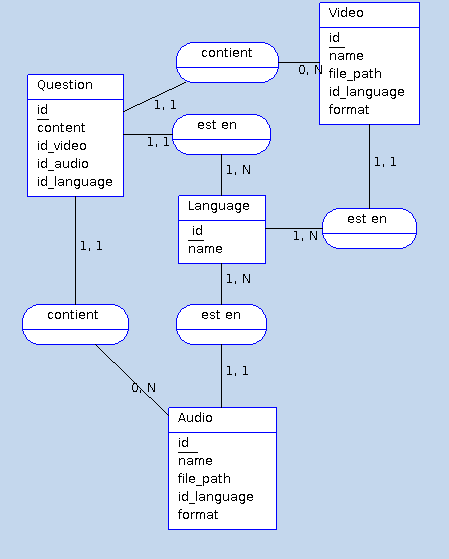
\includegraphics[width=8cm]{./architecture/Merise_BDD.png}}
  \caption{MCD - Base de données}
  \label{MCD} 
\end{center}
\end{figure}


\section{Application tierce : administration}

Nous avons décidé de complètement séparer l'administration de l'application des tests prosodiques, ceci afin que l'administration se fasse beaucoup plus rapidement en ligne de commande depuis un système d'exploitation Linux. Contrairement à l'application principale, cette partie n'est pas multiplateforme. En effet, notre client est habitué à travailler sur ce système d'exploitation, il souhaitait pouvoir administrer l'application avec son outil habituel. De plus, l'utilisation de la ligne de commande nous a permis de créer une administration plus rapide qu'avec une interface dédiée. Cette avantage est important pour notre client qui ne souhaite pas avoir une administration fastidieuse.\\

Cette application tierce sera lancée en ligne de commande en exécutant le fichier \textit{.jar} suivi des paramètres adéquats d'administration. La syntaxe de ces paramètres sera précisée dans la \textit{Javadoc} de l'application.\\

Cette application tierce est composée de deux packages ayant des rôles bien définis que nous allons expliquer ci-contre.

\subsection{Admin}

Ce package est le socle de base de l'application administration.\\
La classe \textit{ProjectProgAdmin} contient tous les appels aux méthodes d'administration de la base de données. C'est à partir de cette méthode que notre client renseignera dans la ligne de commande ses désirs pour manipuler la base de données.\\
La classe \textit{AdminDatabase} contient les méthodes statiques d'administration de la base de données. Elles permettent l'ajout et la suppression des médias et des questions issus d'un fichier texte. De plus, une méthode permet l'affichage dans le terminal du contenu de la base de données.

\subsection{Thumbnails}

Ce package a pour but de générer les thumbnails de chaque vidéo. Ces aperçus sont composés d'une image et d'un gif issus des vidéos. Le package est composé de 4 classes distinctes.\\
La classe \textit{CreationThumbnail} appelle les différentes fonctions qui créent les deux types de thumbnails. Cette classe nous permet de bien appeler les différents objets dans l'ordre voulu.\\
La classe \textit{Picture} est spéciale vu que c'est elle qui crée le thumbnail image mais aussi elle qui appelle la fonction qui coupe la vidéo en différent "BufferedImage". Cette classe utilise les fonctionnalités du projet \textit{Xuggler}.\\
La classe \textit{SliceFrame} découpe la vidéo passée en paramètre dans le constructeur de la classe précédente et crée une liste de "BufferedImage". Ces "images" sont sélectionnées selon la durée renseignée.\\
La classe \textit{Gif} n'a pas été créée par nos soins. En effet, l'auteur Elliot Kroo a créé une classe qui facilite la création d'un gif. Nous avons décidé de prendre sa classe puisqu'elle nous permettait de nous concentrer sur un autre front. De plus, le résultat que nous avons obtenu avec ce système a été satisfaisant.